%\vspace*{-1ex}
\section{Evaluation}
\label{sec-4}

% \subsection{Methodology}
% \label{sec-4-1}

In this section, we evaluate the performance of MediaScope.
%
Although MediaScope's credit assignment algorithm is optimal in a
pseudo-polynomial sense, we are interested in its practical
performance under bandwidth variability.
%
Furthermore, in practice, since query arrival cannot be predicted
ahead of time, the practical performance of MediaScope may deviate
from the optimal.
%
Finally, it is instructive to examine alternative scheduling
mechanisms to quantify the performance benefits of MediaScope's
algorithms.
%
We are also interested in the overhead imposed by MediaScope; since
timeliness is an essential attribute of many queries, system
inefficiencies can impact query completeness.

All our experiments are conducted on a prototype of MediaScope.
%
MSCloud is written mainly in Python; PHP and Python are used for
MSCloudQ web interface.
%
The implementation of MSCloud is about 4300 lines of PHP and Python
code, and MSMobile requires about 1150 lines of C and Java code
(measured using SLOCCount~\cite{sloccount}).
%
% Overall 4093 lines of Python code, and about 200 lines of PHP on
% MSCloud, added/modified 931 lines of java code and 223 lines of C code
% to Medusa on MSMobile side (Counted by SLOCCount).
%

Our experiments use commodity hardware, both for MSCloud and the
mobile device.
%
We use up to 8 Android phones, which are either the Galaxy Nexus or
the Galaxy SIII.
%
MSCloud runs on a Dell XPS 7100 (six-core AMD Phenom II X6 1055T 2.8
GHz processor and 6MB built-in cache).

\begin{figure*}
\centering
\begin{minipage}[t]{5.8cm}
\centering
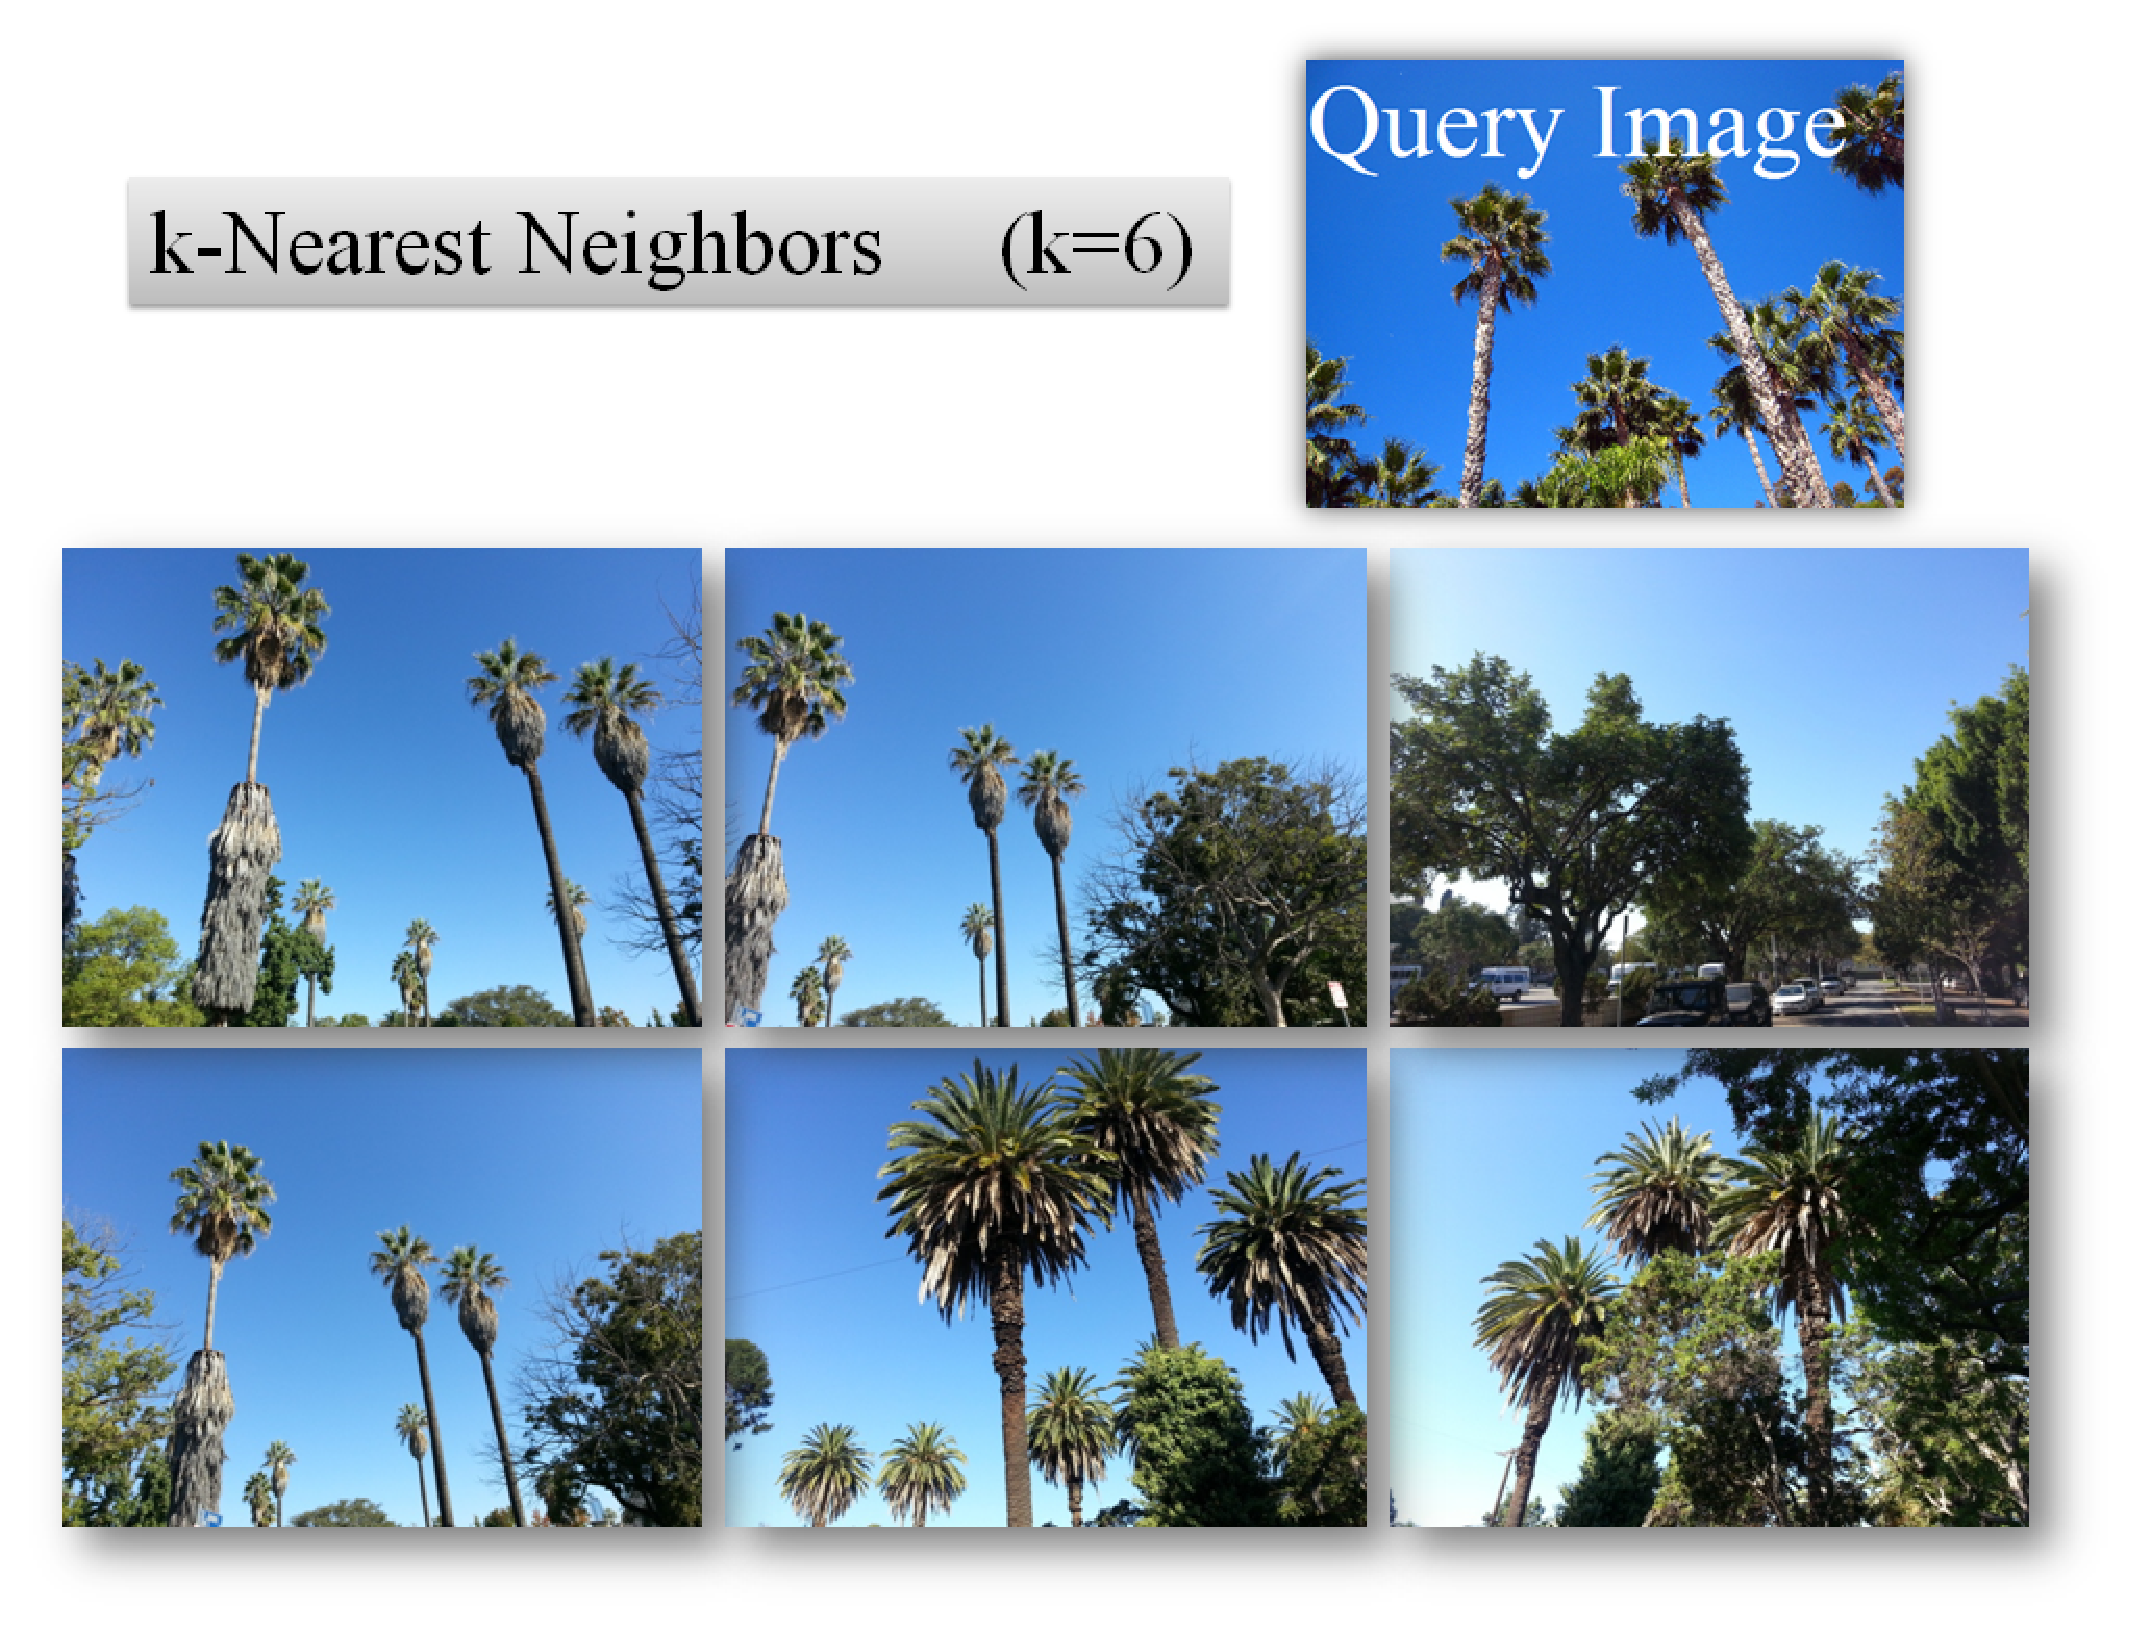
\includegraphics[width = 5.6cm]{pics/1.eps}
\centering \caption{K Nearest Neighbor Result} \label{fig:top_k}
\end{minipage}
\begin{minipage}[t]{5.8cm}
\centering
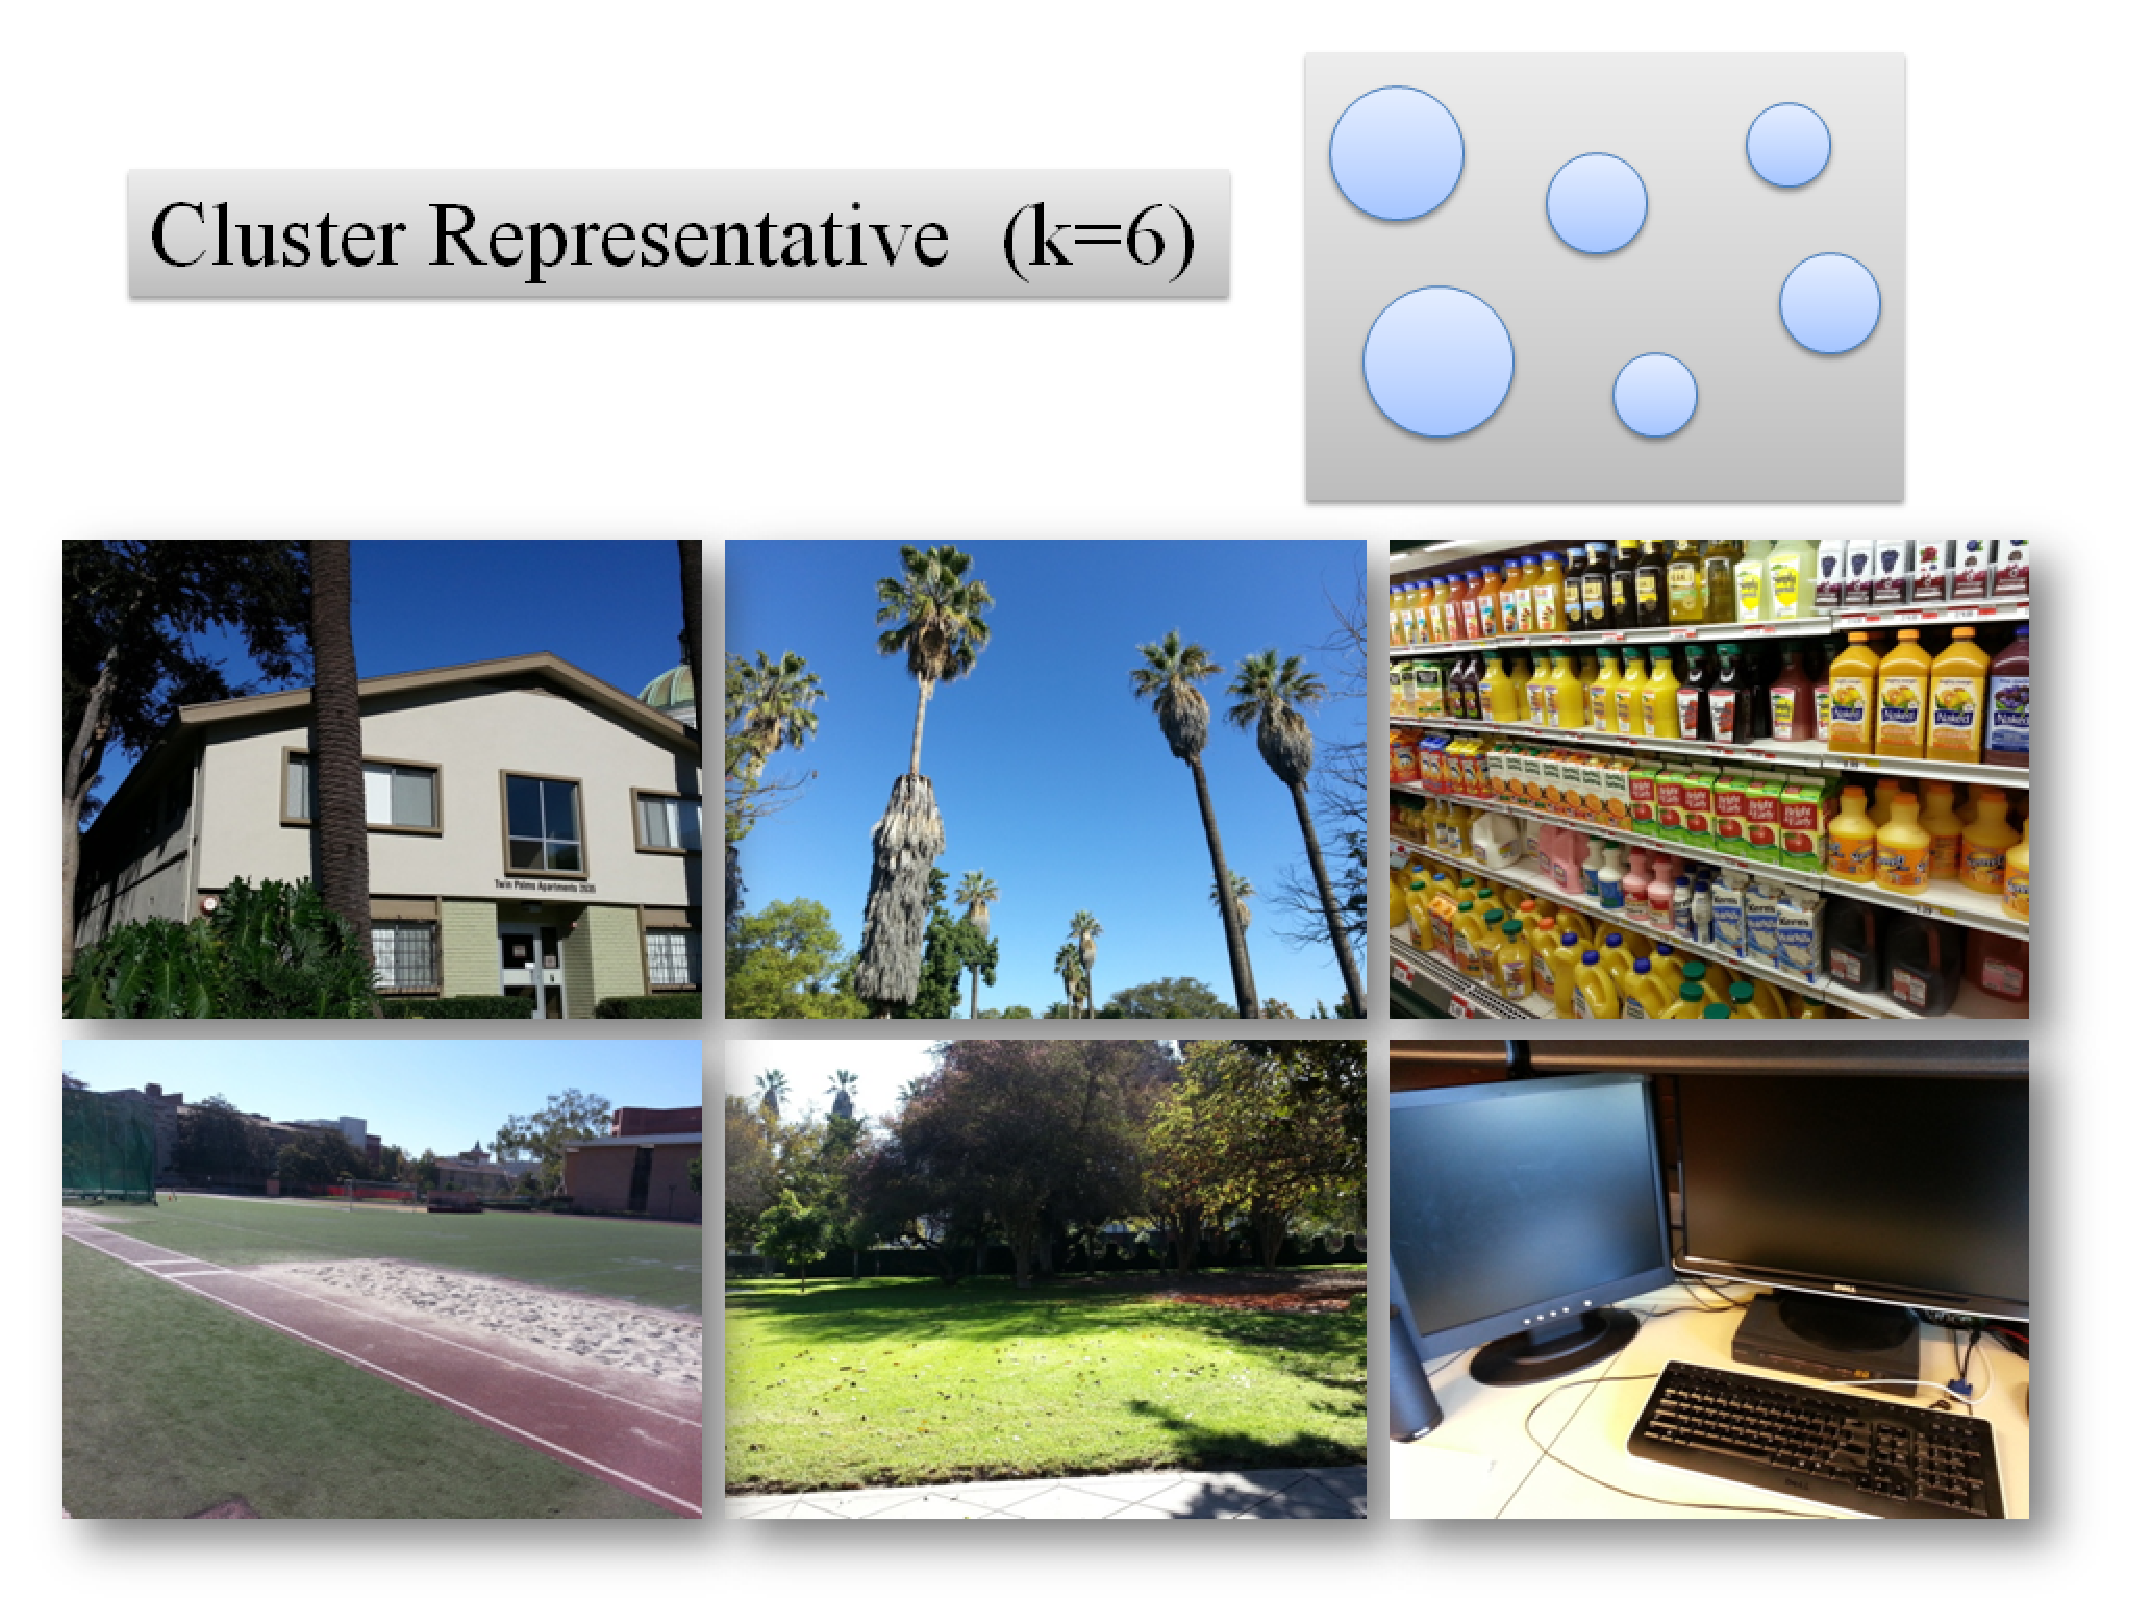
\includegraphics[width = 5.6cm]{pics/2.eps}
\centering \caption{Cluster Representative} \label{fig:cluster_representative}
\end{minipage}
\begin{minipage}[t]{5.8cm}
\centering
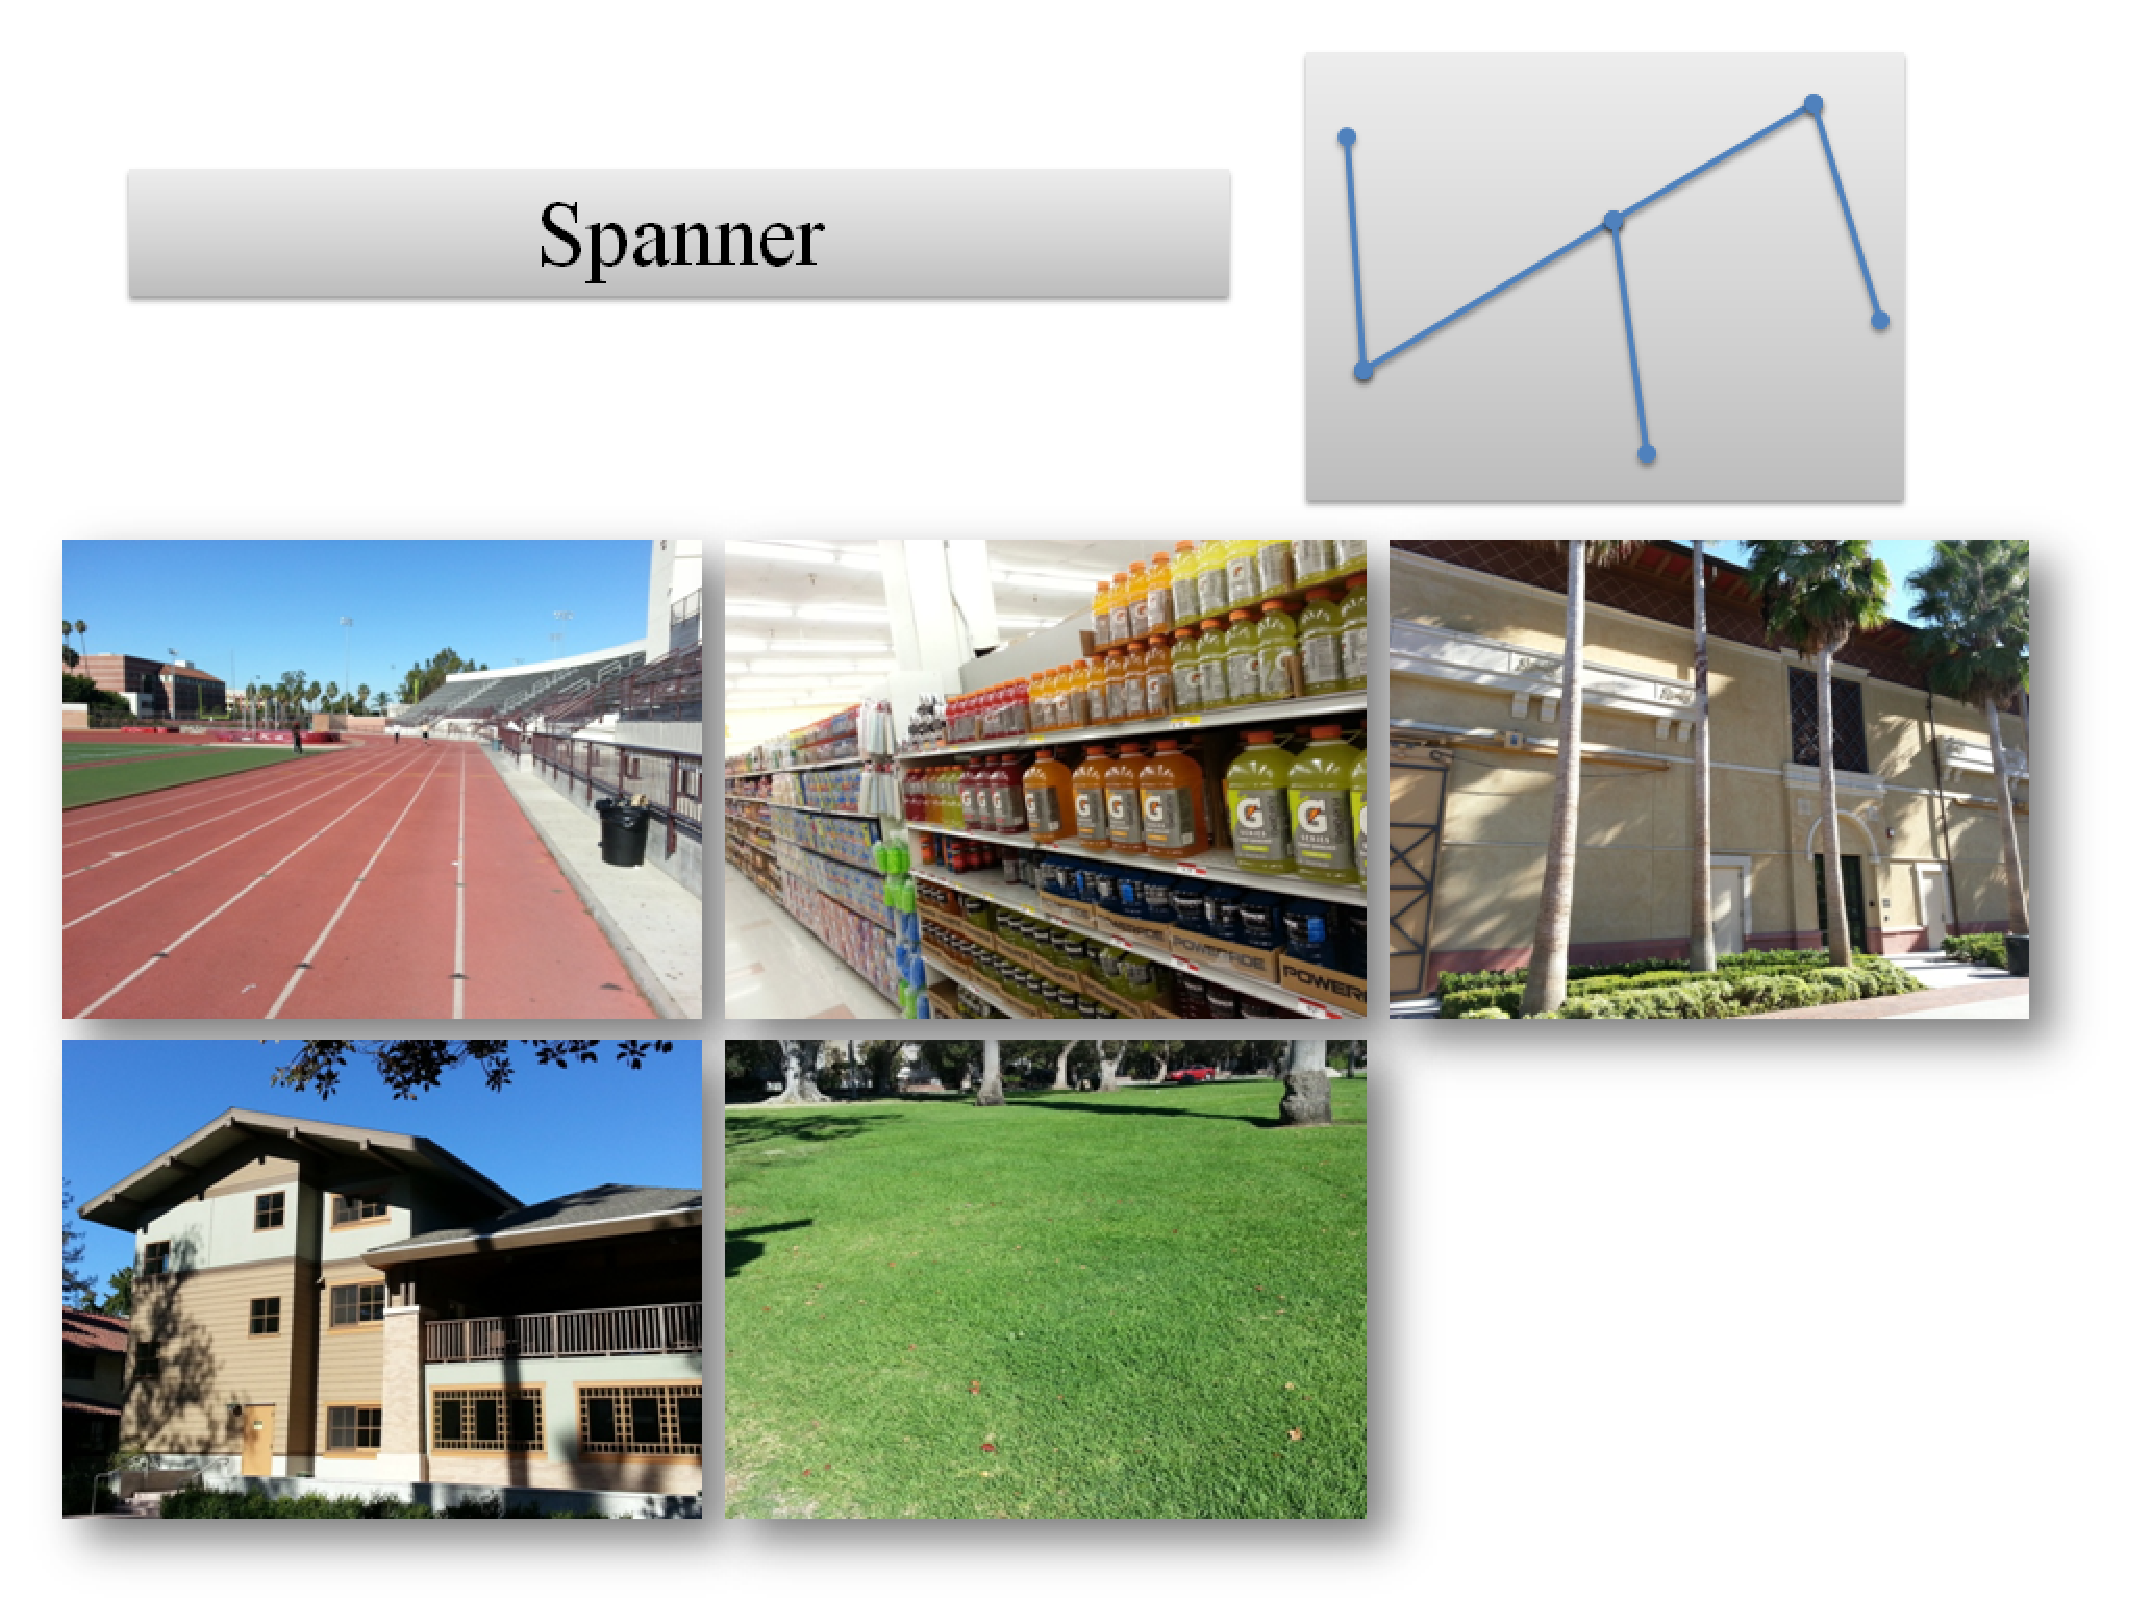
\includegraphics[width = 5.6cm]{pics/3.eps}
\centering \caption{Spanner} \label{fig:spanner}
\end{minipage}
\end{figure*}

Before describing our results, we give the reader some visual
intuition for the usefulness of MediaScope.
%
Figures~\ref{fig:top_k}, ~\ref{fig:cluster_representative},
and~\ref{fig:spanner} show the results of three different queries: a K
nearest neighbor query, a Cluster Representatives query and a Spanner
on a set of six groups of photos: a university campus, a garden, a
view of the sky framed by trees, an athletics track, a supermarket,
and a laboratory.
%
Notice that the cluster representatives query identifies
representatives from each of groups, while the Spanner extracts
qualitatively different pictures, while the K nearest neighbor query
extracts matching images as we might expect.
%
%In contrast,... \ramesh{Will fix after top-K}

% We run our $K Cluster Representative$ query and $Spanner$ query on the photo set with  total 175 feature vectors (some from short videos), and results are shown on Figure~\ref{fig:sample}
%  }

%\vspace*{-0.75ex}
\subsection{Query Completeness}
\label{sec-4-2}

In this section, we evaluate query completeness in the presence of
concurrent queries.

\mypar{Metrics and Methodology.}
%
Our metric for query completeness is the total credit associated with
all the query results successfully uploaded before their timeliness
bounds.
%
We evaluate several \emph{query mixes} (described below), with
different concurrent queries of query types that arrive at different
times and have different timeliness bounds.
%
These queries are all posed on 320 images captured on 8
mobile devices.
%

Our experiments are conducted as follows.
%
For each query mix, we first compute the results of each query and the
credit assigned to each result object.
%
This computation yields a \emph{trace}, on each mobile device, of
objects, their associated credits and the arrival time.
%
We use this trace to replay the credit-based scheduling algorithm
during repeated runs and report the average of 10 runs.

This trace-based methodology is also useful in comparing MediaScope's
credit-based scheduling algorithm (henceforth, \emph{MSC}) with
several alternatives.
%
For each alternative, we replay the trace for that particular
scheduling algorithm.
%
We consider the following alternatives: an \emph{Omniscient} algorithm
that knows about future query arrivals; a \emph{Max Credit First
  (MCF)} that always selects the object with a maximum credit to
upload; a \emph{Round Robin (RR)} that allocates bandwidth fairly to
each concurrent query so that, in each round, the object with the
highest credit from each query is uploaded; and an \emph{Earliest
  Deadline First (EDF)} scheduler that always schedules that object
with the earliest timeliness bound first, breaking ties by credit.
%
The Omniscient algorithm demonstrates the benefits of lookahead, while
each of the other algorithms has at most one of MSC's features
(timeliness-, credit-, and bandwidth-awareness).

In our experiments,  each mobile device contains a number of images
taken with its camera.
%
These images are naturally of different sizes because they have
different levels of compressibility.
%
Furthermore, we make no attempt to control network variability; upload
bandwidths in our experiments vary and MSC estimates upload bandwidth
by measuring the average speed of the last upload (MSC's algorithm
needs uses this estimate for $t(o)$).

%
% In our evaluation, 8 Android phones each has captured roughly 40 images in advance for querying. We design several series of concurrent queries, including all the query types we implemented. For each series of concurrent queries, we record the starting time and deadline of each query, as well as selected objects with its credits for repeating the process of uploading for $10$ times. For each generated series of concurrent queries $\mathbb{Q}$, total credit received $c(\mathbb{Q})$ will be considered as the (only? fairness?) matric.

% We will compare our scheme described in \ref{sec-3-2-2} against a variety of alternative approaches, namely \textit{Max Credit First}, \textit{Earliest Deadline First} and \textit{Round Robin}. Max Credit First (MCF) scheme always picks the one with the maximum credit to upload; Earliest Deadline First (EDF) scheme uploads the object with the earliest deadline; \textit{Round Robin} allocates bandwidth fairly to all the ongoing queries, in each round, every query will be uploaded one media object. The last competitor acts as a theoretical upper bound, which knows all the future queries $\mathbb{Q}$ at time $0$ and uploads based on the optimal schedule, we call it $\textit{Optimal with Full Knowledge} (FULL)$.

\begin{figure*}[t]
  \begin{minipage}{0.32\linewidth}
    \centering \epsfig{file=pics/different_queries.eps, width=0.95\linewidth}
    % \vspace{-1mm}
    \caption{Different Query Mixes by Size}
    %\vspace{-6mm}
    \label{fig:different_queries}
  \end{minipage}
  \begin{minipage}{0.32\linewidth}
    \centering \epsfig{file=pics/different_times.eps, width=0.95\linewidth}
    % \vspace{-1mm}
    \caption{Different Query Mixes by Timeliness Bound}
    %\vspace{-6mm}
    \label{fig:different_times}
  \end{minipage}
  \begin{minipage}{0.32\linewidth}
    \centering 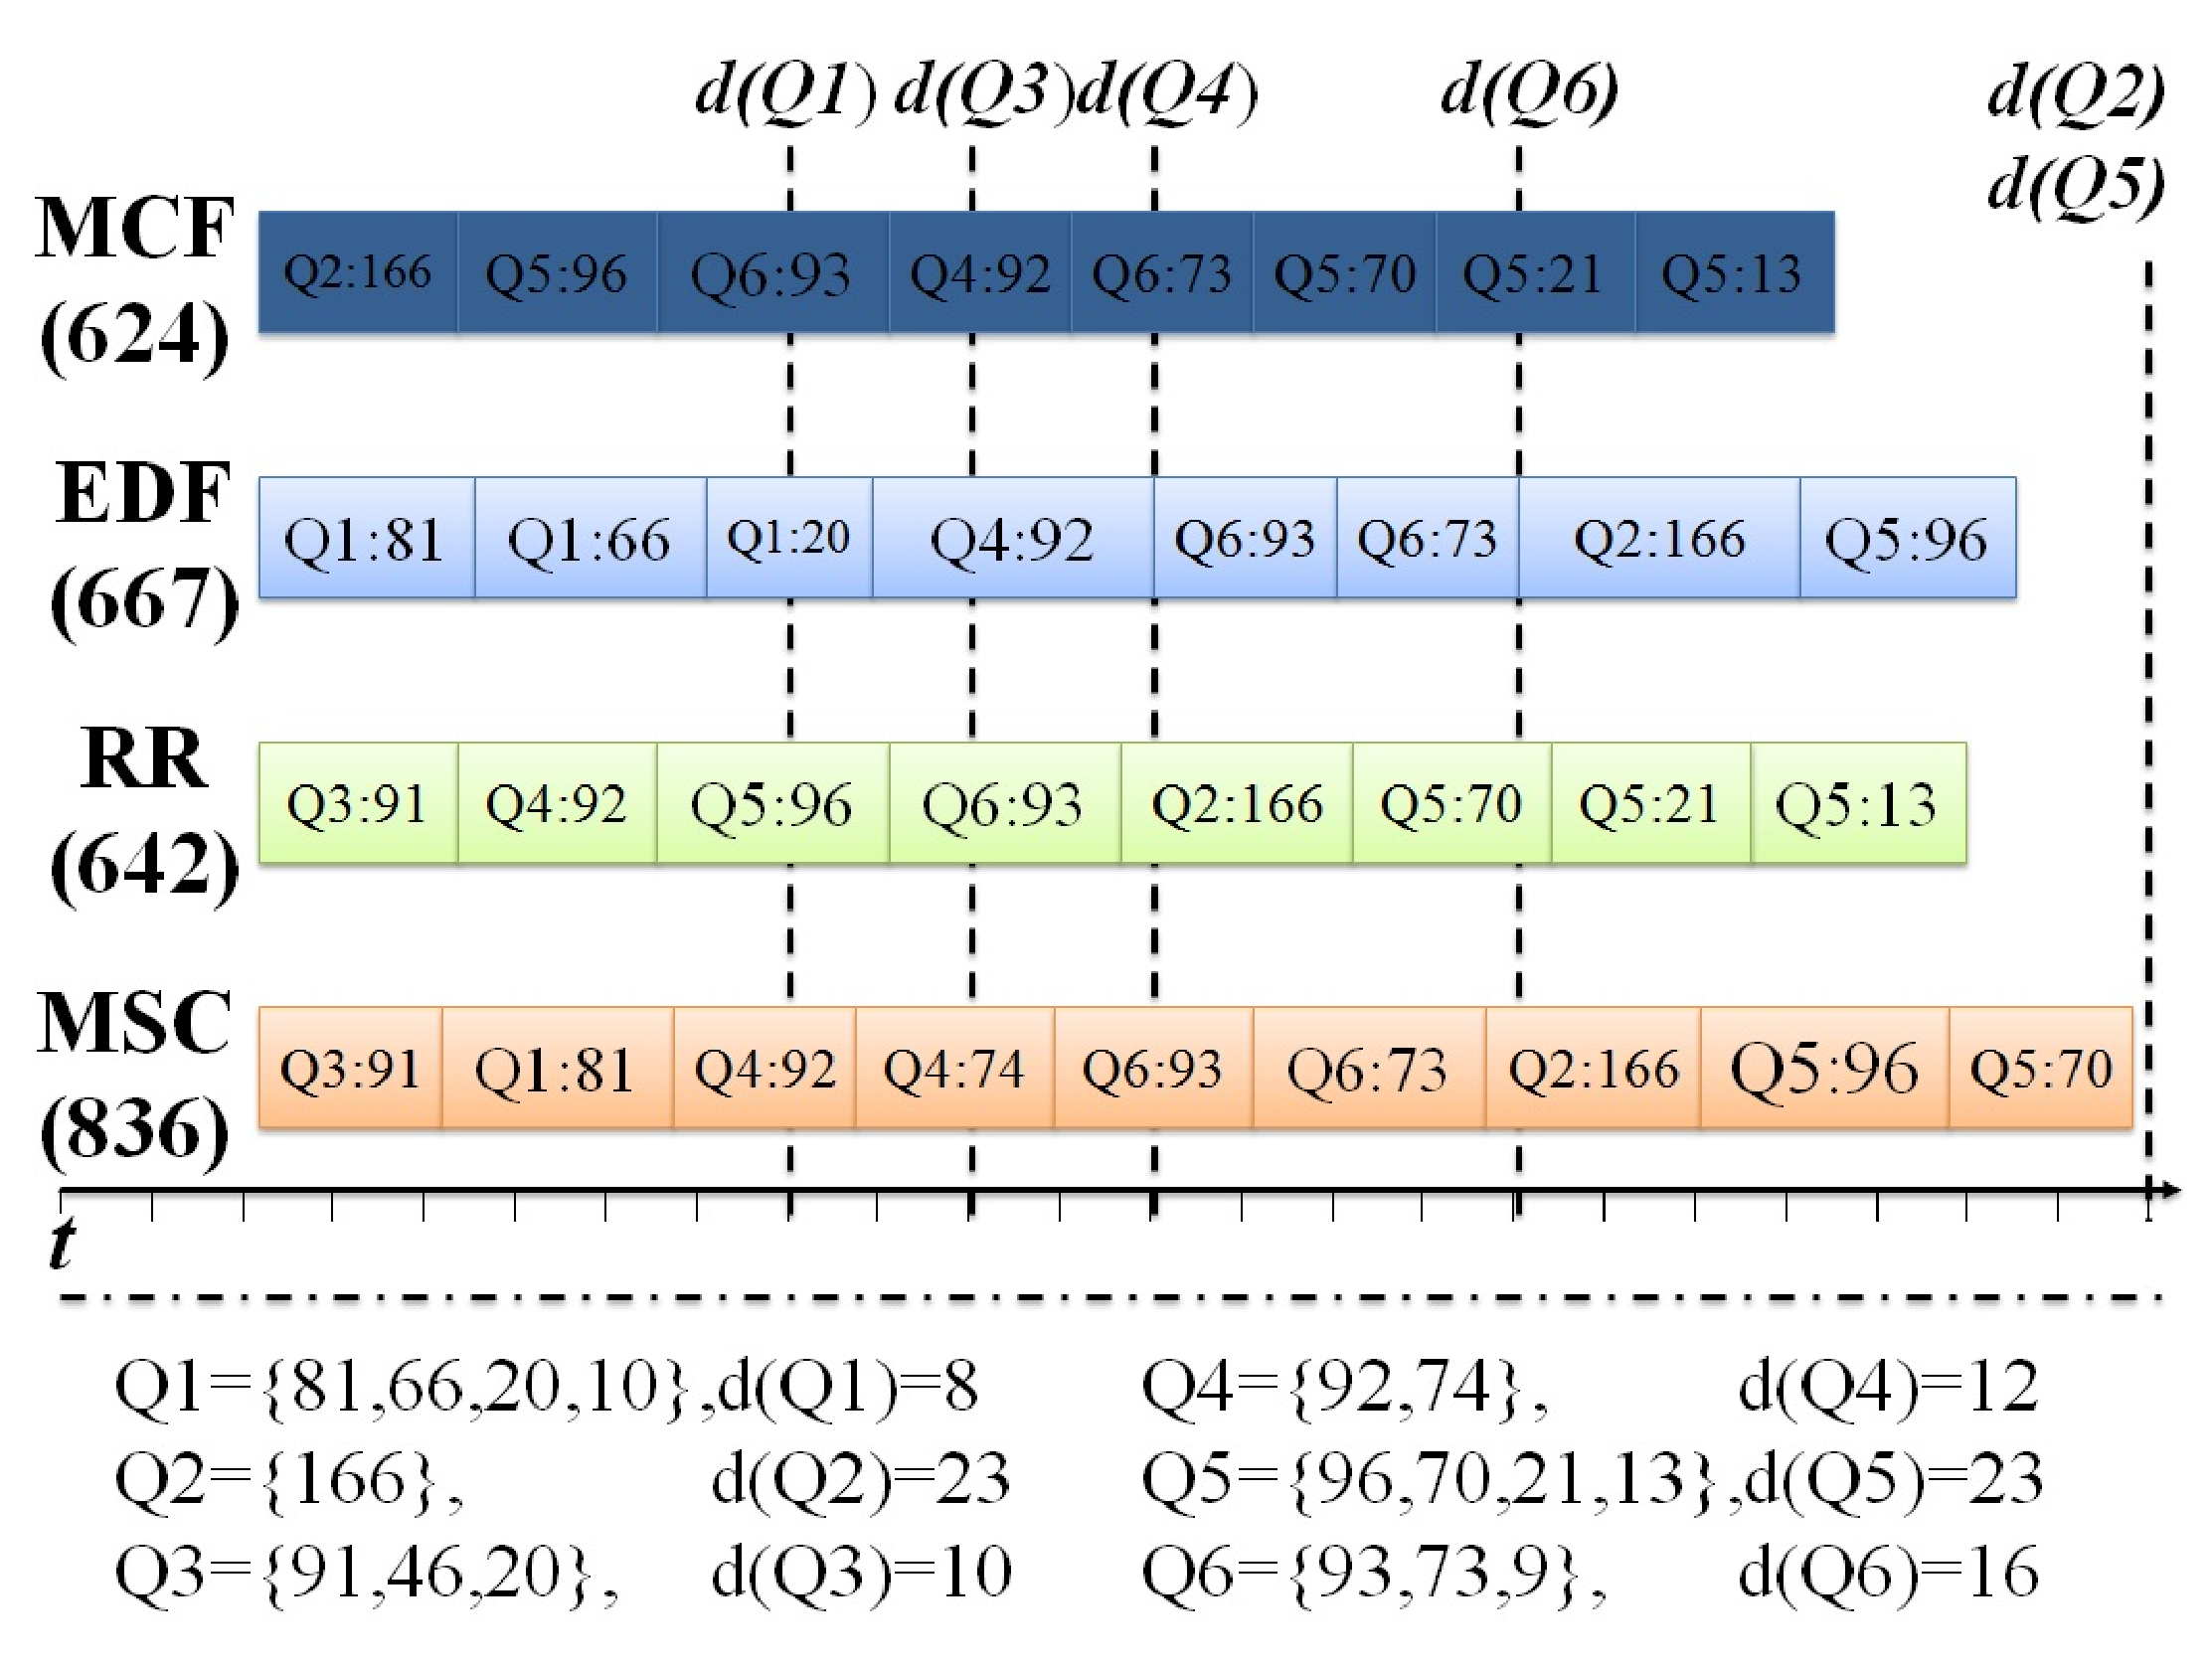
\epsfig{file=pics/timeline.eps, width=1.05\linewidth}
    %\vspace{-6mm}
    \caption{Sample Schedule Timeline}
    %\vspace{-6mm}
    \label{fig:timeline}
  \end{minipage}
\end{figure*}

\mypar{Results.}
%
Our first experiment compares the performance of these alternatives
for three different query mixes with different types of queries.
%
The first mix contains 4 queries, namely, 1 Top-K, 1 Spanner, 1
Cluster Representative and 1 Common Interest.
%
All the queries arrive at the same time but with different timeliness
bounds; thus, in this experiment there are no future arrivals and we
do not evaluate the Omniscient algorithm.
%
The second mix adds one more Cluster Representative query to the first
one, and the third is generated by adding one more Common Interest
query.
%
In each query mix, each query is assigned the same total credit.
% the total query completeness score for a given query mix can be
% obtained by multiplying the number of queries in the mix by 1000.

% All the query assign selected objects with credits up to 1000.
% %
% So in this setting the maximal credits we can get is the query number
% times 1000.
% %

Figure~\ref{fig:different_queries} shows the performance of various
schemes.
%
MSC achieves at least 75\% completeness across all three query mixes,
and its performance improves by 5\% as the number of queries increases
from 4 to 6.
%
Although a 75\% completeness rate seems pessimistic, we remind that
reader than MSC is optimal, \emph{so no other scheduling scheme could
  have done better than this}; in other words, for this query mix,
this is the best result that could have been achieved.

Furthermore, MSC outperforms other schemes significantly.
%
The superior performance of MSC comes from its
timeliness-awareness, credit-awareness, and adaptivity to available
bandwidth.
%
By contrast, approaches that lack one or more of the features have
much lower completeness rates.
%
Thus, EDF does not take into account an object's credit, and thus
might waste bandwidth on objects with an early deadline but small
credit; on average, EDF achieves 55\% completeness.
% \ramesh{Fix.}\xing{percentage added}
%
RR is unaware of timeliness constraints, but uploads the result
objects for each query in a round-robin fashion.
%
It is comparable in performance to EDF, achieving 52\% completeness on
average. % \ramesh{Fix}\xing{percentage added}
%
RR's poor performance arises from two factors: first, because it
ignores timeliness constraints, it uses transmission opportunities by
sometimes transmitting objects which could have been deferred without
violating data timeliness bounds; second, RR gives equal transmission
opportunities to queries, even though, on a given mobile device, one
query may contain objects with far more credit than another query.
%
MCF improves upon RR in the second aspect, in that it always transmits
the object with the highest credit first; in so doing, it achieves an
average completion rate of 59\% and is significantly better than EDF
and RR. % \ramesh{Fix}. \xing{percentage added}
%
However, MCF is still noticeably worse than MSC, primarily because MCF
ignores timeliness constraints and sometimes transmits objects that
could have been deferred without violating timeliness bounds.

% The reason is, RR achieves fairness on each phone, but not globally.
% %
% Consider the extreme case where $Q_1$ assigns several important
% objects to $P_1$, on the other hand $Q_2$ and $Q_3$ assign not
% important objects to phone 1, it is obvious that $P_1$'s local
% fairness is not efficient since in this case $Q_1$ should get more
% resources.
% %
% The result of MCF is not bad, since it greedily earn max credit in
% every round.
% %
% MCF is an effective scheme but anyway it has not consider deadline so
% in the worst case, MCF can perform as bad as only $50\%$ of optimal
% scheme.
% %
% Our scheme performs the best in all the settings, uploaded roughly
% $75\%$ of the total credits.
% %
% In addition, as the number of concurrent queries increasing, our
% scheme performs better compared to other competitors.
% %
% The reason can be explained by the value of ``planning'': when there
% is lacking the opportunity of planning, simply MCF would be an
% effective solution (consider two extreme cases, when there is no
% concurrency and there are bursty queries); however when there are
% modest concurrent queries, our scheme can leverage the advantage of
% planning.
%

In order to get more insight into the relative performance of these
schemes, we consider variants of the 6-query mix which have different
combinations of arrival rates and deadlines.
%
Figure~\ref{fig:different_times} plots the results of these experiments.

In the first query mix, three of the six queries arrive first with the
timeliness bound of 20 seconds.
%
The remaining three queries arrive within three seconds, but have a
relatively tight timeliness bound of 6 seconds.
%
In this sense, they \emph{interrupt} the first set of queries.
%
This query mix is designed to demonstrate the benefits of
timeliness-awareness.
%
In this somewhat adversarial setting, MSC still outperforms other
schemes but has a much lower completeness rate of about
60\%. % \ramesh{Add.} \xing{percentage added}
%
RR performs poorly, but EDF performs comparably to MCF; this is not
surprising because EDF is timeliness-aware.
%
Even so, EDF does not perform as well as MSC because it ignores credit
values and uploads objects with lower credits unnecessarily.

% Fig. \ref{fig:different_times} shows the same queries of above
% experiment of 6 queries, but this time we vary the arriving time and
% the deadline of such queries. The first setting which we call it
% ``interrupted'' setting, where 3 queries come first, with late
% deadline of 20 seconds, while another 3 queries come 3 seconds later
% but with relatively tight deadline of 6 seconds. The latter 3
% queries act as ``interruptor'', and this setting is evaluating which
% scheme can handle these interruptors well. MCF is always a strong
% scheme, however, we see EDF performs also good in this case because
% when the interruptor came in it, it stopped to upload interruptor's
% objects. Our scheme is still the best among all the schemes.

In the second query mix, 6 queries with the same timeliness
requirement arrive in a staggered fashion, with each query arriving
three seconds after the previous query.
%
This illustrates a setting where queries arrive frequently but the
arrivals are not synchronized.
%
In this setting, MSC achieves a completeness rate of nearly 80\%, and,
not surprisingly, MCF comes quite close with a completeness rate of
71\%.
%
Since all queries have identical timeliness bounds, it is not
surprising that a credit-aware scheme like MCF performs well.
%

The third query mix represents a complex pattern where queries arrive
at different times and have different deadlines.
%
For this mix, the performance advantages of MSC are clear, since this
mix requires a scheduling scheme to be both credit and
timeliness-aware.

% but all queries have the same timeliness bound.
% \xing{In the second query mix, 6 queries come one by one, 3 seconds after previous query, and of the same timeliness bound of 6 seconds.}
% %
%  \xing{In a setting that there would be frequent future queries coming in,} This mix is designed to illustrate the importance of credit awareness,
% and one might expect that, in this setting, MCF would perform best.
% %
% Indeed, we find that MCF achieves a completion rate of about 71\% on
% average. \ramesh{Fix.} \xing{percentage added}
% %
% In this setting, MSC is comparable to MCF; by design, it uploads the
% highest credit objects for the first set of queries, and then adapts
% its uploading schedule when the second set of queries arrives.

% Surprisingly, EDF also performs well in this setting...
% \ramesh{Will re-write this once the new experiments are in}

% The second setting sets all the queries with the same deadlines, similar to interrupted setting, three queries come 3 seconds later. It is clear that if all the queries are of the same deadline, then MCF would be the optimal solution. However, our scheme might be dangerous in this setting, because our scheme tries to plan the uploading but incoming queries might ``disagree'' the original plan and make our scheme ``regret'' about previous decision. But from the result we can see our scheme performs as good as the optimal one, MCF. The reason is, our scheme not only do the theoretical optimal schedule, but also switch the selected one with the maximum credits but of the same deadline. With this simple modification, our scheme would hardly ``regret'' about this decision when the future queries come in.

% The third setting is the most complicated one and with the most value
% of planning, where queries' arriving time are different as well as deadlines. In this
% setting, MCF, EDF and RR all are not comparable to our scheme.
% \ramesh{Will rewrite this when the new results are in.}

Finally, for all these query mixes (Figure \ref{fig:different_times}),
MSC is comparable to the Omniscient scheme, which knows the arrival
times of different queries.
%
Intuitively, because MSC continuously adapts its transmission
schedules when new queries arrive, it can make a different decision
from Omniscient only at the times when queries arrive.
%
To be more precise, say a new query arrives at time $t$: Omniscient
might have scheduled an upload of an object for the new query starting
at time $t$, but MSC has to wait until the object being uploaded at
$t$ finishes, before it updates its schedule.
%
This difference can be fixed by adding \emph{preemption} to the
scheduler, aborting the current transmission if it does not have the
highest priority; we have left this to future work.
% \ramesh{Xing,
%   please check.} \xing{generally correct. but in the extreme case, our scheme may `regret' about already uploaded ones: say, if I know there would be a bursty queries coming soon with higher credits than what I have, I don't need to do any 'schedule', or say any 'planning' is bad idea; except for MCF, MCF is good for bursty, by bursty I mean lots of incoming queries with higher credits...}

% it can at most be worse than
% Omniscient by the credit associated with one object (the one being
% transmitted

% we added the ``cheating scheme'', FULL, which know all the incoming
% queries at time 0. But in all three settings, we see our scheme's
% performances are pretty close to it, showing that optimal scheduling
% based on current queries is indeed a good intuition for the real case
% where new queries will join at any time, at least for the modest
% concurrent queries case.

To get some more insight into the differences between the scheduling
algorithms, Figure~\ref{fig:timeline} plots the timeline of decisions
made by these algorithms for the 6-query mix when all queries arrive
at the same time.
%
The figure clearly shows that MSC is better able to use the available
time to carefully schedule uploads so that completeness is maximized;
MCF, having uploaded objects with high credits is unable to utilize
the available time because the timeliness bound for the remaining
objects has passed.
%
EDF performs comparably to MCF, but, because it is credit-unaware,
misses out on some transmission opportunities relative to MSC (e.g.,
MSC uploads Q3:91 first, but EDF does not).

\camera{
In summary, our approach bridges the availability gap by extracting
relevant photos and images dynamically from participating devices.
%
The approach hinges on the observation that feature space similarity
can be used to determine relevant media objects, and that image
features are an extremely compact representation of the contents of an
image.
%
However, it is well-known that content based information retrieval
exhibits a \emph{semantic gap}~\cite{gap}: feature-based similarity
matching is oblivious to the semantic structures within an image, so
the matching may not be perfect.
%
In these cases, we rely on additional filtering by human intelligence
(e.g., in our examples, the security officer, or the reporter).
%
To put it another way, our approach may not always give the
  right answer, because of the semantic gap. To properly evaluate our
  approach, we need to conduct a user study. This is because, for example,
  determining whether the results of a spanner query really span a
  given corpus can be highly subjective. We have left this user study
  to future work.}

% why MSC scheme is better than the
% alternatives, taking into account of both credit and deadline.
% %
% MCF considers only credits and when important object's timeliness
% bound expires, the remaining objects are all with small credits; on
% the other hand, EDF wastes bandwidth on objects with low credits.
%
% \ramesh{Will rewrite this after it has been updated.}\xing{in this
% particular example EDF is not so bad, but clearly it missed one
% opportunity of uploading Q3=91.
% %
% You can see that our scheme faced the same problem, but MSC gave up
% Q3=91 for Q4=92 for conservative, which is smart.}
%

%\vspace*{-0.75ex}
\subsection{System Overhead}
\label{sec-4-3}

\mypar{Latency.}
%
Because MediaScope attempts to satisfy timeliness constraints, the
efficiency of its implementation can impact query completeness; the
less overhead incurred within the system, the greater the query
completeness can be.
%
To understand the efficiency of our system, we profiled the delays
within the various components of MediaScope (Table~\ref{tab:factor}).
%
In an earlier section, we have discussed the cost of feature and frame
extraction: these operations are not performed in the object retrieval
path, so do not affect query timeliness.

%
% In \mscope, we measure the end-to-end speed from task posting to file uploaded to MSCloudDB, generally the average speed for uploading a  1.5MB or so image is about 466KB/s with WiFi and 408KB/s with ATT 4G in our area.

% We also find that when file size goes larger, the speed increases some. To understand the reason behind this, we measure each component of \mscope that could cause the latency other than the network speed. The results are shown in ~\ref{tab:factor},

\begin{table}
  \footnotesize
    \centering
    \begin{tabular}{ lc}
    \toprule
    & Average Latency (ms) \\
    \midrule
    MSCloud to Medusa & 131 \\
    C2DM (send-to-receive) & 150 \\
    Task Execution & 67 \\
    Upload Scheduling & 46 \\
    Medusa to MSCloud Image Transfer & 67 \\
    \bottomrule
    \end{tabular}
    \caption{System Communication and App Running Overhead}
    \label{tab:factor}
\end{table}
%
As this table shows, the latency incurred for most components is
modest; C2DM notifications take less than 1/6 second, and the
communication between MSCloud and Medusa takes about 1/8 second.
%
Other components are under 70 ms.
%
%\jyr{data update, task execution time}
% By far the most latency consuming component is task execution within
% Medusa; in some sense, we pay this performance penalty for building
% upon a general-purpose system for crowd sensing.
% %
% In the near future, we expect to optimize Medusa task execution to
% reduce this latency overhead.

Finally, latency within the MSCloudQ query engine is also moderate
(Table~\ref{tab:overhead}).
%
Even in our relatively un-optimized implementation, most components of
query processing take less than 100ms, with the only exception being
the download of feature vectors from MSCloudDB; we plan to optimize
this component by caching feature vectors in memory.

These overhead numbers suggest that our current prototype
may be able to sustain timeliness bounds of 10s or lower.
%
Indeed, some of our experiments in the previous section have used 6s
timeliness bounds.

% \jyr{In our relatively unoptimized implementation, Feature Vector Filtration and downloading takes slightly more time, however, these middle component overhead can be further reduced by caching in the future}

\begin{table}
  \footnotesize
    \centering
    \begin{tabular}{lc}
    \toprule
     & Average Latency (ms) \\
    \midrule
    Query Parsing & 24 \\
    Feature Vector Download & 138 \\
    Medusa Server Interpretation & 68 \\
    Spanner & 89 \\
    K Clusters & 52 \\
    K Nearest Neighbor & 11 \\
    Query Result Response & 54 \\
    \bottomrule
    \end{tabular}
    \caption{System Function Components Overhead}
    \label{tab:overhead}
\end{table}

\mypar{Energy.}
%
The other component of overhead is energy expenditure.
%
Frame extraction and feature extraction can take up to a second, or
more, of CPU time.
%
The energy cost, on a Motorola Droid (measured using a power meter),
of frame extraction is 57 $\mu$Ah, and of feature extraction
(including resizing) is 331 $\mu$Ah.
%
We believe these energy costs are still reasonable: for feature
extraction to consume even 10\% of the Droid's battery capacity, a
user would have to take more than 400 photos!
%

% \section{overhead}
% \jyr{We give a sample result in Figure~\ref{fig:sample}


% \subsection{System Overhead}
% \label{sec-4-3}

% \subsubsection{Metrics}

% In \mscope, we measure the end-to-end speed from task posting to file uploaded to MSCloudDB, generally the average speed for uploading a  1.5MB or so image is about 466KB/s with WiFi and 408KB/s with ATT 4G in our area.

% We also find that when file size goes larger, the speed increases some. To understand the reason behind this, we measure each component of \mscope that could cause the latency other than the network speed. The results are shown in ~\ref{tab:factor},
% \begin{table}
%     \centering
%     \begin{tabular}{ | l | l | l |}
%     \hline
%     Drawback Factors & Average Latency(ms) \\ \hline
%     Server Notification & 231 \\ \hline
%     C2DM(send-to-receive) & 251 \\ \hline
%     Task Exec & 2103 \\ \hline
%     Upload scheduling & 46 \\ \hline
%     Server-to-Server File Feteching  & 67 \\ \hline
%     \end{tabular}
%     \caption{Potential Drawback Factors For uploading Speed}
%     \label{tab:factor}
% \end{table}
% It's  easy to find that major drawback factor is task execution which takes about 2s, other factors such as Server-to-Server Notification as well as C2DM message delay are some other major factors that cause \mscope upload speed performance degrading.


% \subsubsection{Results: Overhead}
% \label{sec-4-4}
% In the end, we measure  the latency of the component in MSCloudQ, the results are show in \ref{tab:overhead}
% \begin{table}
%     \centering
%     \begin{tabular}{ | l | l |}
%     \hline
%     System Components & Average Latency(ms) \\ \hline
%     Query Parse & 612 \\ \hline
%     Optimization(Spanner) & 89 \\ \hline
%     Optimization(K Clusters) & 52 \\ \hline
%     Optimization(Top K) & 11 \\ \hline
%     \end{tabular}
%     \caption{System Components Overhead}
%     \label{tab:overhead}
% \end{table}
% From the results, one major delay is Query parsing, which we think depends on what script you run in background. Other parts are neglectable.






% \subsubsection{Metrics}
% System overhead:

% \begin{itemize}
% \item time to upload a small file end-to-end: use Wifi and cellular network
% \item breakdown of latency:
% \begin{itemize}
% \item where is the latency going? (Medusa server, notification, medusa
%       phone etc.)
% \end{itemize}
% \end{itemize}


% \subsubsection{Results: Overhead}
% \label{sec-4-4}






%original
% \subsection{System Overhead}
% We evalute the media processing on Galaxy SIII with specification: Quad-core 1.4 GHz Cortex-A9, Android OS, v4.0.4, with 8 MP, 3264x2448 pixels, 1080p@30fps.
% \subsubsection{Frame Extraction}
% To see how efficiency our frame extraction algorithm, we test with multiple videos of different duration, more specifically, we separate videos by the duration: 30s, 60s, 120s, and for each duration, phone takes around 10 videos by itself, we also set the extraction frequency as follows: 8Hz, 4Hz, 2Hz, 1Hz, 0.5Hz, 0.25Hz, 0.125Hz, by Hz we mean the number of frames extracted in 1 second. In the Figure \ref{fig:frame}, we show the average total extraction time with different frequency.
% \begin{figure*}[!t]
% \centering {
%     \subfigure[Average 30s Videos  Processing Time]{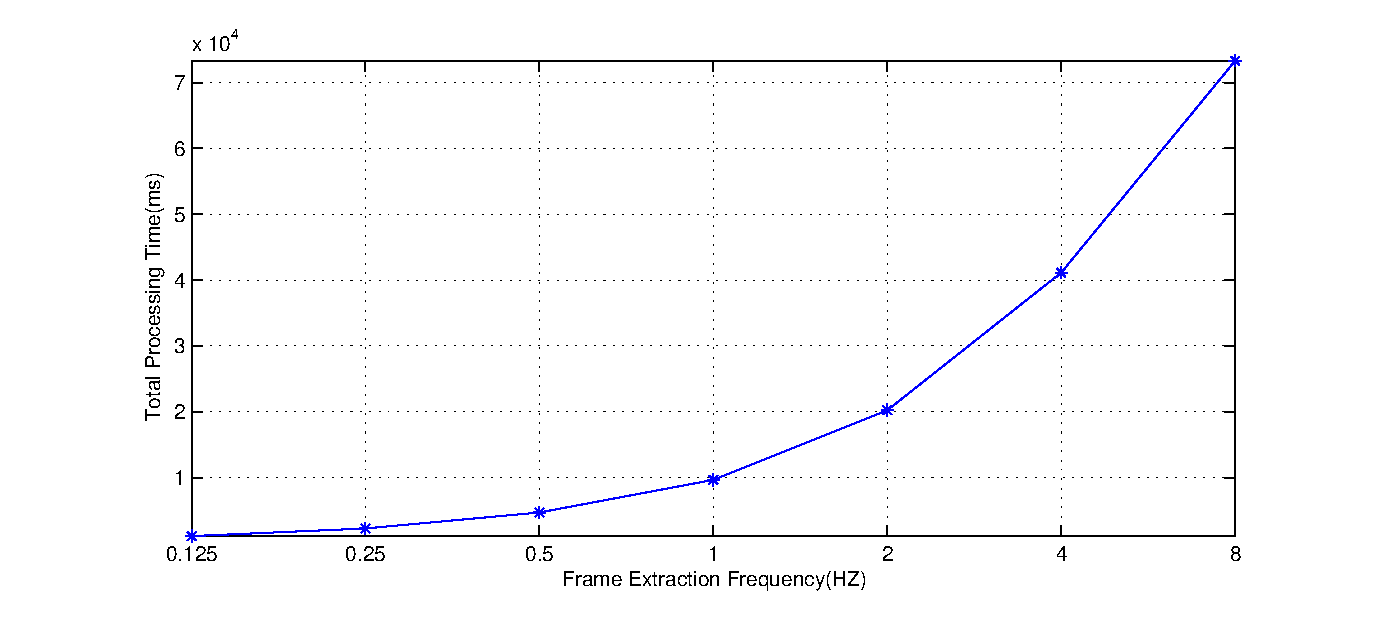
\includegraphics[width=2in]{pics/30s_frame.eps}\label{fig:3_1}}
%     \hfil
%     \subfigure[Average 60s Videos  Processing Time]{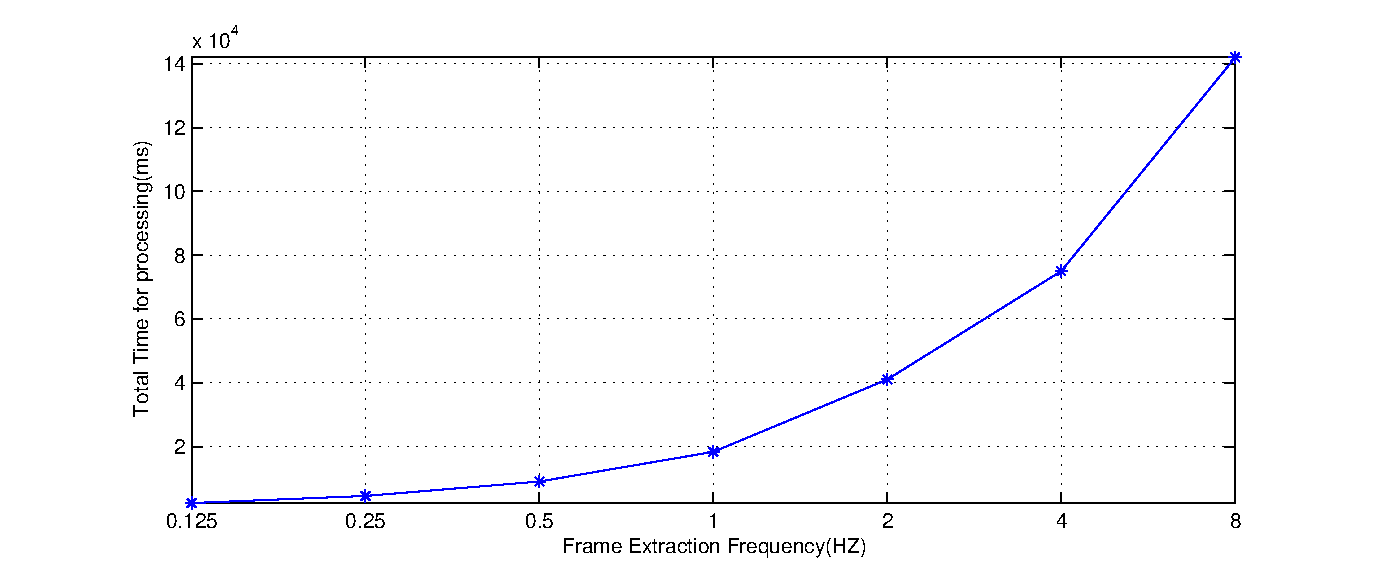
\includegraphics[width=2in]{pics/60s_frame.eps}\label{fig:3_2}}
%     \hfil
%     \subfigure[Average 120s Videos  Processing Time]{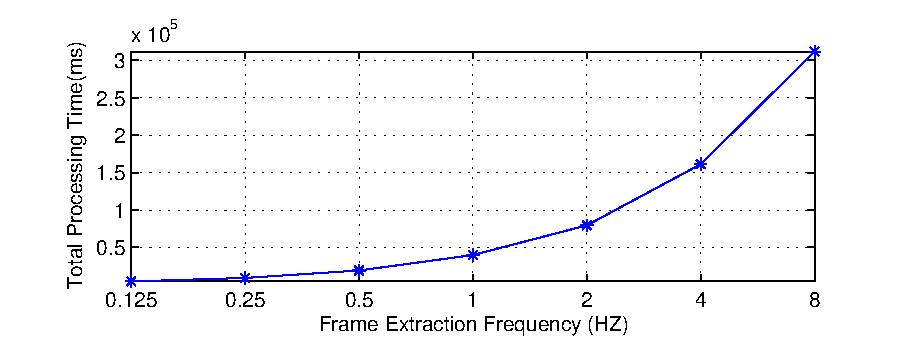
\includegraphics[width=2in]{pics/120s_frame.eps}\label{fig:3_3}}
% }
% \vspace{-1mm}
% \caption{Average Video Frame Extraction Time For Different Duration and Frequency}
% \vspace{-6mm}
% \label{fig:frame}
% \end{figure*}
%
% .
% \begin{enumerate}
%     \item Given a video, extract frames at different rate: 0.5Hz, 1Hz, 2Hz,... get the average extracting time for each rate
%     \item Fix a rate, extract different size video, see if there is any affects for different size video
% \end{enumerate}
% \subsubsection{Feature extraction}
% For the feature extraction of single image, we need to consider two aspects of cost, first, the cost of resizing, second, the cost of feature extraction of resized image. We use Galaxy SIII for this cost evaluation, we took about 300 photos of different kinds of scene with phone's own camera, and rescale them to different size, and record different component time for processing each file, and get the average time. We can see from the figure that...
% \begin{enumerate}
%    \item Given an image data base, resize all the images into  a fixed size. Do different feature extraction algorithm, and compare these algorithm's average extracting time
%    \item resize image data base into different size(100x100, 200x240, 300x400...), compare the average time for these sizes for different algorithm
% \end{enumerate}
%
% \subsubsection{Communication Measurement}
% End2End uploading speed estimate, give a uploading command from server and wait the end of file uploading, see the time. We vary
% the file size: a small photo to a large video. Compare WiFi(ENL WiFi) and cellular network (OPTIONAL: minus the real file uploading time from phone to server, we can see the overhead, how does the overhead vary?)
%
% \subsection {Background Media File Processing Performance}
% There might exists a scenario that media file process is running while  people are using their phones, we should ensure people's experience not much affected by our background processing.
%
% The experiment, we need to show the cpu and memory occupation by this thread.
%
% \subsection{Simpler System Comparison}
% Take away some part of our system, see how results perform;
%
% \subsection{Dynamic vs. Static Uploading Scheme}
% In fact, we have two kinds of scheme for file uploading, since the optimization result is sensitive, one way is to dynamically re-optimize and update the uploading list to phone, another is that push an enough long list to the phone and let phone do static uploading. The drawback of dynamic uploading is that the task assigning and killing process wastes a lot of resources, the results would be bad comparing to static uploading.
%
% We should show the reason why we choose static uploading finally
%
%
%
% \subsection{ Evaluation of  Concurrent Queries}
% \begin{enumerate}
% \item Set up and replay concurrent queries to compare with other uploading schemes: 1) round robin; 2) max credit first; 3) earliest deadline first;
% \item Compare to the ``optimal result'': run concurrent queries and record necessary parameters, use the information as facts in real world, apply scheme to get the ''Optimal Result''
% \end{enumerate}
%
% \subsection{Evaluating Overall Results}
% \begin{enumerate}
% \item Show the output performance with some intuitive metric;
% \item Compare with other possible phone media retrieval scheme;
% \end{enumerate}
%
% \subsection{Robustness and Scalability}
% \begin{enumerate}
% \item Handling burst of concurrent queries;
% \item Scales to \bf{N} phones, see how server performs, any degrading?
% \end{enumerate}

